%{\bfseries COMMENT: It doesn't seem right to have so little text on the threat when there is so much on countermeasues.}

%{\bfseries COMMENT: you don't have any references for challenge-response?}


\begin{figure*}
	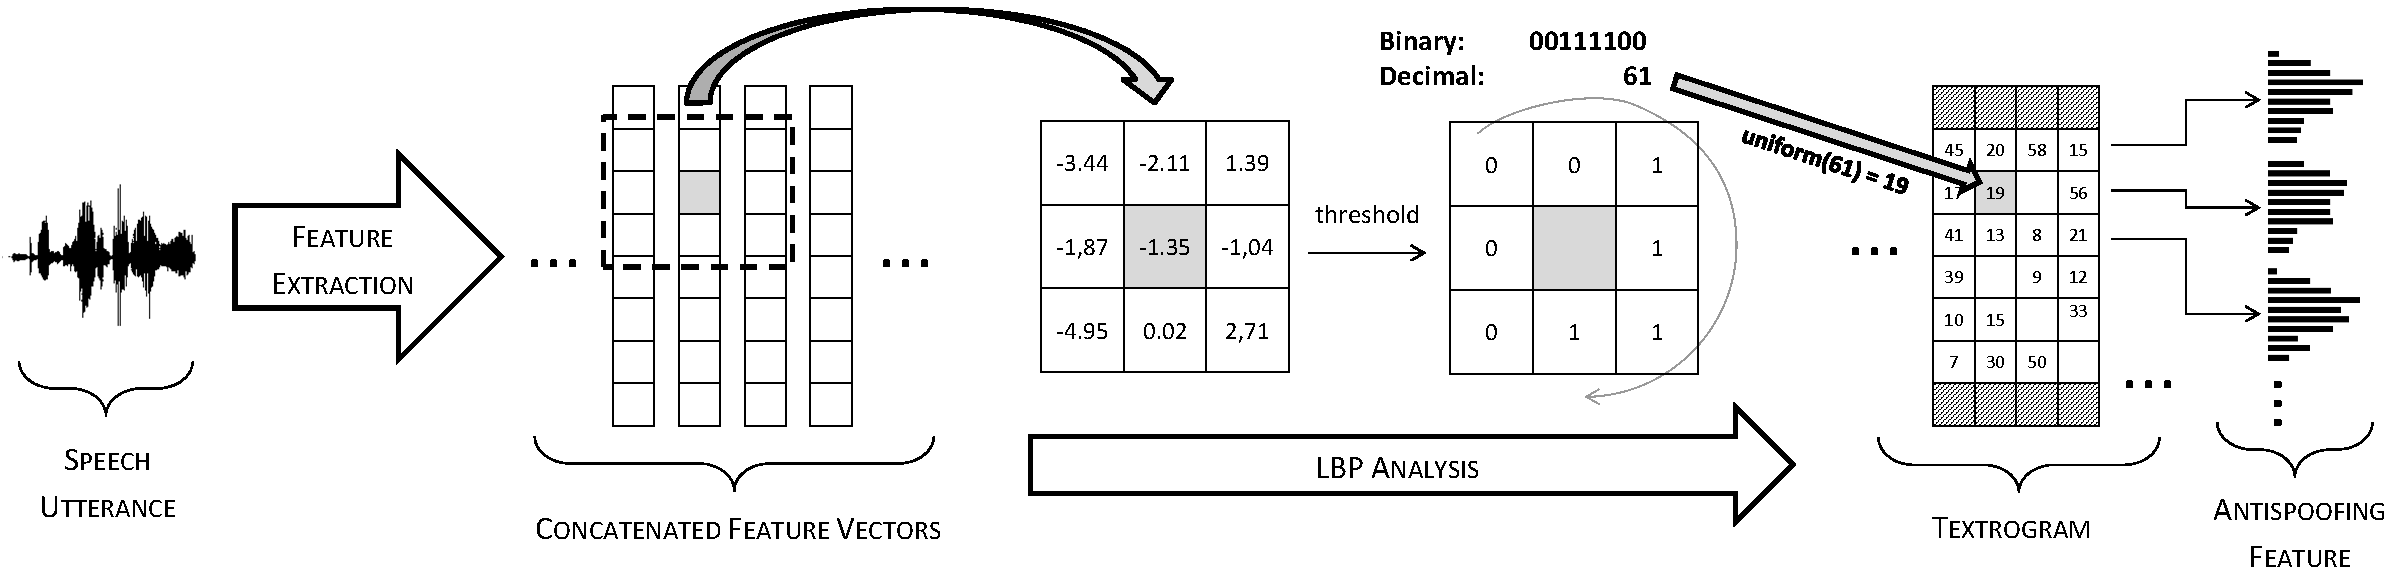
\includegraphics[width=1\linewidth]{Figs/LBPfeature.pdf}

	\caption{Schematic diagram of forming a feature vector in the LBP-based countermeasure.}
	\label{fig:LBPfeature}
\end{figure*}




Given that only little work has investigated attacks, it is not surprising that the work in anti-spoofing is similarly limited.  
One obvious approach involves challenge-response systems which require the speaker to utter a prompted ad hoc phrase~\cite{Petrovska1998}. 
Challenge-response mechanisms are a form of passive countermeasure; more active countermeasures have also been proposed.
One approach involves the storing of previous access attempts and their comparison to new attempts~\cite{Shang2010}. A somewhat similar technique is proposed in~\cite{Wu2014}, where the authors compare spectral bitmaps between access trials and previously stored recordings in text-dependent scenario.
The detection of high similarity was shown to serve as an effective means of identifying replay attack, albeit in a rather constrained scenario.
%The experiments showed that this method caused a decrease in EER in  most of the cases, however, this method is useless if there were no previous access trials with a given recording. 

Other methods 
%work in investigated the use of channel noise statistics as a means of detecting replay attacks.  These methods 
essentially aim to detect the presence of an unexpected channel, i.e. channel artefacts indicative of recording and replaying.
Two such algorithms were reported in~\cite{Wang2011} and show reductions in 
% The authors proposed two variants of their countermeasure, and they managed to decrease the EER from
an equal error rate (EER) from 40\% to 10\% with a baseline GMM-UBM system subjected to replay attacks.

\subsection{Far-field recording detection}

Villalba and Lleida~\cite{Villalba2011} investigated a method which involves  channel-detection, too, but in a peculiar way. The authors noticed that since many logical and physical access based ASV systems can reasonably expect close-talk speech, and since some recordings will be made surreptitiously or at-distance, the detection of far-field speech can serve as an effective countermeasure.  

In their experiments, each recording, both from the training and the testing datasets, was additionally described using the following 12 parameters:
\begin{itemize}
\item spectral ratio -- the ratio between
the signal energy from 0 to 2 kHz and from 2 kHz to 4 kHz.  The average value of the spectral ratio for the speech segment was calculated using speech frames only. By using this value the authors hoped to detect the flattening of the spectrum due to noise and reverberation, caused by far-field recording;
\item low frequency ratio -- ratio between the signal energy from 100 Hz to 300 Hz and from 300 Hz to 500 Hz, calculated using speech frames only. This value was said to be useful for detecting the effect of the loudspeaker on the low part of the spectrum of the replayed signal;
\item total signal modulation index; and
\item nine sub-band modulation indices, for sub-bands: 1kHz-3kHz, 1kHz-2kHz,
2kHz-3kHz, 0.5kHz-1kHz, 1kHz-1.5kHz, 1.5kHz-2kHz, 2kHz-2.5kHz, 2.5kHz-3kHz and 3kHz-3.5kHz.
\end{itemize}

According to the authors of the algorithm, the envelope of the far-field recording has higher local minima mainly due to the additive noise, what should result in lower modulation indices. Sub-band modulation indices were added to detect far-field recordings disturbed with coloured noises, because according to the authors, a narrow-band noise can affect only a small frequency band and it might not have a noticeable effect on the total modulation index.  


Villalba and Lleida's work showed that their far-field recording detector was able to detect replay samples with 90\% recognition accuracy, this is why we decided to test it in our work with a large speaker database and various ASV systems.
% ; therefore they extracted 12 parameters describing the envelope and, based on them, trained a binary SVM classifier in order to discriminate far-field speech from close-talk speech. The authors claimed that they reached the far-field recognition rate of more than 90\%.


\subsection{Local binary patterns}

%{\bfseries COMMENT: Probably not a great idea to write so much about this one technique (our own) whereas you allocate only a very small amount of text to other work (by other authors).  I suggest to greatly reduce and to merge with the material above in one section on previous work.}

Another method, proposed in~\cite{Alegre2013a}, uses local binary patterns (LBP) technique. It is based on the hypothesis that modifications made through spoofing disturb the natural 'texture' of genuine speech. This technique was adopted from a standard texture analysis approach, known in image processing~\cite{Ojala2002}, to a 2-dimensional 'image' of a speech utterance, where the image is a mel-scaled cepstrogram appended with dynamic features. 

The standard LBP operator is a non-parametric 3x3 kernel which assigns a binary code to each pixel in an image according to the comparison of its intensity value to that of its eight surrounding pixels~\cite{Ojala2002}. This procedure is illustrated in Fig.~\ref{fig:LBPfeature}.  A binary value of '1' is assigned when the intensity of neighbouring pixels (here feature components) is higher, whereas a value of '0' is assigned when neighbouring pixels are of lower or equal intensity. Each pixel is thus assigned one of $2^8=256$ binary patterns.

LBPs are determined for each pixel in the mel-scaled cepstrogram thus resulting in a new matrix of reduced dynamic range, here referred to as a 'textrogram'.  The textrogram captures short-time feature motion beyond that in conventional dynamic parametrisation.  The LBP-based countermeasure is based on concatenated histograms formed from the pixel values across each row in the textrogram.  The histograms are individually normalised and their resulting bin values are stacked vertically to obtain a new vector in the same manner as GMM mean-vectors are stacked to form supervectors.  


This method turned out to be  highly effective for artificial signals, yielding 0\% EER for the five tested ASVs, very effective for speech synthesis attacks (EER values below 1\%) and quite effective for voice conversion -- EERs less than 7\%. Considering the fact that the LBP-based countermeasure hardly relies on prior knowledge on the attack, in this work we decided to try to use it also as a countermeasure against replay attacks.


%{\bfseries COMMENT:  I would restructure this section.  Having learned that we ought to be concentrating on replay, the subsections on voice conversion and synthesis seem misplaced.  Better to have a general section on spoofing, to introduce replay, voice conversion and speech synthesis and then the comparison.}


\subsection{Aim of this work}

This paper aims at analysing threat of replay attacks when using large speaker databases and most effective speaker verification systems, and compare it with the threat of other spoofing algorithms: voice conversion and speech synthesis. The impact of acoustic environment and playback devices on performance of speaker verification systems will be also investigated. 

Due to lack of real replay recordings (e.g., similar to the MOBIO corpus collected in real environment~\cite{Khoury2013a}) we had to use artificial setup of replay environment, however, using impulse responses calculated using real playback hardware and real acoustic environments. 

This work will also verify the effectiveness of replay detection, using two previously described replay countermeasures: 
\begin{itemize}
\item the far-field detector (from here on in referred to as FFD) described in~\cite{Villalba2011}, which had been shown to be effective in detecting far-field recordings, and 
\item the local binary patterns-based detector (from here on in referred to as LBP), described in~\cite{Alegre2013a}, which yielded satisfactory results for a variety of attacks (artificial signals, speech synthesis and voice conversion).
\end{itemize}
Therefore, we are going to identify a relative threat of replay using the state-of-the-art ASV systems and two replay countermeasures.
